\documentclass[a4paper]{article}

%% Language and font encodings
\usepackage[english]{babel}
\usepackage[utf8x]{inputenc}
\usepackage[T1]{fontenc}

%% Sets page size and margins
\usepackage[a4paper,top=3cm,bottom=2cm,left=3cm,right=3cm,marginparwidth=1.75cm]{geometry}

%% Useful packages
\usepackage{amsmath}
\usepackage{amsfonts}
\usepackage{graphicx}
\usepackage{subcaption}
\usepackage[colorinlistoftodos]{todonotes}
\usepackage[colorlinks=true, allcolors=blue]{hyperref}

\graphicspath{ {figures/} }

\title{Possible Inconsistency in Maximum Likelihood Calculation of Ancestral States}
\author{Shaw, Matsen, Minin}

\begin{document}
\maketitle

%comments from Erick:
% >  This is great!
% > - would be great to have all the calculations showing the "refinement" structure written out for the various tree structures (just done by hand and scanned is just fine) 
% > - I think of the "refinement" as a partition, so perhaps rather than "empty refinement" we have a "single-element partition"
% > - in order to interpret the site patterns I need to figure out in what order the leaves are labeled
% > - how is ell calculated?
% > - on the numerical sanity check, it doesn't seem clear that the branch lengths can be different than the inferred ones-- they can!
% > - re "general case", agreed though I don't think that we need numerical optimization of branch lengths in a set of a branch length partition-- we can just get the optimal branch length directly. Namely, for each branch, we know all hidden states (given that we are in a set of a partition) and so can count the number of mutations across that branch. From there we have a simple likelihood function, which either has an optimal in the interior or on the boundary of the partition.

\renewcommand{\arraystretch}{1.2} % because otherwise exponents get eaten by \hline

\section{Ancestral state reconstruction using maximum likelihood}

\subsection{The usual story}

We have observed character data $\mathbf{y}=[y_1,\ldots,y_n]\in\mathcal{Y}^n$ and corresponding unknown ancestral states $\boldsymbol\xi=[\xi_1,\ldots,\xi_n]\in\Xi^n$.
Both $\mathcal{Y}$ and $\Xi$ are discrete sets.
Without loss of generality, assume $\mathcal{Y}=\Xi=\{0,1\}$.
For a topology $\tau$ and branch lengths $t$ we form the likelihood
\begin{equation}
\label{eq:full_likelihood}
L_n(\mathbf{y};\boldsymbol\xi, \tau, t) = \prod_{i=1}^{n} \ P(y_i, \xi_i | \tau, t).
\end{equation}
In particular, we are interested in
$$
(\hat{\boldsymbol\xi}, \hat{\tau}, \hat{t}) = \arg\max_{\boldsymbol\xi, \tau, t} \ L_n(\mathbf{y};\boldsymbol\xi, \tau, t),
$$
which we call the maximum likelihood values of the parameters $(\boldsymbol\xi, \tau, t)$.

Since the number of elements in $\boldsymbol\xi$ grows with that of the observed data $\mathbf{y}$, the typical approach to estimate these parameters involves computing the marginal likelihood
\begin{equation}
\label{eq:marginal_likelihood}
\tilde{L}_n(\mathbf{y}; \tau, t) = \sum_{\boldsymbol\xi} \ L_n(\mathbf{y};\boldsymbol\xi, \tau, t).
\end{equation}
and maximizing over the topology and branch lengths to obtain
$$
(\hat{\tau}, \hat{t}) = \arg\max_{\tau, t} \  \tilde{L}_n(\mathbf{y}; \tau, t).
$$
The values $\hat{\boldsymbol\xi}$ are then calculated conditional on these estimates.
More likely in practice we fix a topology $\tau$ and use this marginalization approach to compute $(\hat{\boldsymbol\xi}, \hat{t})$.

\subsection{Joint maximization}

One tantalizing approach is to do away with the marginalization and the two-step maximization, directly estimating the maximum likelihood parameters from the full likelihood in \eqref{eq:full_likelihood}.
We can perform this iteratively, now computing a profile likelihood
\begin{equation}
\label{eq:profile_likelihood}
L_n'(\mathbf{y};\tau, t) = \max_{\boldsymbol\xi} \ L_n(\mathbf{y};\boldsymbol\xi, \tau, t)
\end{equation}
and estimating the topology and branch lengths via
$$
(\hat{\tau}, \hat{t}) = \arg\max_{\tau, t} \ L_n'(\mathbf{y};\tau, t)
$$
while using $\hat{\boldsymbol\xi}$ from \eqref{eq:profile_likelihood} as an estimate for $\boldsymbol\xi$.

\textbf{Claim to prove}: Is it obvious that this particular iterative approach can be done? In other words, do $(\hat{\boldsymbol\xi}, \hat{\tau}, \hat{t})$ from \eqref{eq:profile_likelihood} correspond to those of \eqref{eq:full_likelihood}? I believe since $\Xi$ is a discrete set that this is true, but it may be worth a more rigorous argument.

\subsection{Site pattern formulation}

Now, since $\mathcal{Y}$ and $\Xi$ are discrete sets, we define unique site patterns $\mathbf{s}=[s_1,\ldots,s_q]\in\mathcal{S}$ and ancestral state categories $\mathbf{z}=[z_1,\ldots,z_q]\in\mathcal{Z}$ such that
\begin{align}
L_n'(\mathbf{y};\tau, t) &= \max_{\boldsymbol\xi} \ L_n(\mathbf{y};\boldsymbol\xi, \tau, t) \\
    &= \max_{\boldsymbol\xi} \ \prod_{i=1}^{n} \ P(y_i, \xi_i | \tau, t) \\
    &= \max_{\mathbf{z}} \ \prod_{j=1}^{q} \ P(s_j, z_j | \tau, t)^{n_j} \label{eq:site_pattern_likelihood}
\end{align}
where $n_j$ is the number of observations in the sample where site pattern $s_j$ was seen.
Since $\mathcal{S}$ and $\mathcal{Z}$ are also discrete sets, the value of each factor $P(y_i, \xi_i | \tau, t)$ will be maximized at one or more values of $\xi_i$, though independent of $i$ given $j$.
This independence allows us to group factors by those where $\xi_i$ equals $z_j$ so that $P(s_j, z_j | \tau, t)$ is maximized.

\textbf{Example:} This might be a good time for a toy example showing this for a very simple topology.

\subsection{The case of infinite data}

We are now interested in the properties of the objective function being maximized in \eqref{eq:site_pattern_likelihood}.
Let
$$
L_n''(\mathbf{s};\mathbf{z},\tau,t) = \prod_{j=1}^q \ P(s_j, z_j | \tau, t)^{n_j}
$$
so that
$$
\max_{\boldsymbol\xi} \ L_n(\mathbf{y};\boldsymbol\xi, \tau, t) = \max_{\mathbf{z}} \ L_n''(\mathbf{s};\mathbf{z},\tau,t).
$$
Now assume $n$ observations were generated from a model with parameters $(\tau^*, t^*)$.
We have
\begin{align}
\frac{1}{n} \log L_n''(\mathbf{s};\mathbf{z},\tau,t) &= \sum_{j} \frac{n_j}{n}\cdot \log P(s_j, z_j | \tau, t) \\
  &= \sum_{j} \frac{n_j}{n}\cdot [\log P(s_j | \tau, t) + \log P(z_j | s_j, \tau, t)].
\end{align}
In the limit of infinite data we see
$$
\frac{1}{n} \log L_n''(\mathbf{s};\mathbf{z},\tau,t) \rightarrow \sum_{j} P(s_j | \tau^*, t^*) \cdot [\log P(s_j | \tau, t) + \log P(z_j | s_j, \tau, t)]
$$
and that, since $z_j$ appears only in the last term, the log of \eqref{eq:site_pattern_likelihood} in the same limit is proportional to
\begin{align}
\frac{1}{n} \log L_n'(\mathbf{y};\tau, t) &= \max_{\mathbf{z}} \ \frac{1}{n} \log L_n''(\mathbf{s};\mathbf{z},\tau,t) \\
    &\rightarrow \max_{z_1, \ldots, z_q} \ \sum_{j} P(s_j | \tau^*, t^*) \cdot [\log P(s_j | \tau, t) + \log P(z_j | s_j, \tau, t)] \\
    &= \sum_{j} P(s_j | \tau^*, t^*) \cdot [\log P(s_j | \tau, t) + \max_{z_j} \ \log P(z_j | s_j, \tau, t)]. \label{eq:site_pattern_profile_likelihood_mean}
\end{align}

\textbf{A note on terminology:}  While we are passing to the limit of infinite data, we don't actually \emph{need} infinite data for these results to be striking. Another way of considering the above is what would happen if we knew the ``truth,'' i.e., the true generating topology and branch lengths.

\subsection{Showing inconsistency}

For clarity, define \eqref{eq:site_pattern_profile_likelihood_mean} as
$$
J(\tau, t; \tau^*, t^*) = \sum_{j} P(s_j | \tau^*, t^*) \cdot [\log P(s_j | \tau, t) + \max_{z_j} \ \log P(z_j | s_j, \tau, t)]
$$
where $(\tau, t)$ are the estimands and $(\tau^*, t^*)$ are the fixed, generating parameters.
For data generated from $(\tau^*, t^*)$, if there exist estimands $(\tau,t)\neq(\tau^*,t^*)$ where
$$
J(\tau, t; \tau^*, t^*) > J(\tau^*, t^*; \tau^*, t^*)
$$
then we have a possible inconsistency, and the maximum likelihood parameters obtained in this manner may not conform to the truth in the limit.
The issue with this approach is that we do not guarantee any estimation procedure will recover the values $(\tau, t)$.
We may show a stronger, more suggestive result if for $\tau'\neq\tau^*$ we have
\begin{equation}
\label{eq:inconsistency_inequality}
J(\tau', \hat{t}_1; \tau^*, t^*) > J(\tau^*, \hat{t}_2; \tau^*, t^*)
\end{equation}
with $\hat{t}_1$ and $\hat{t}_2$ estimated by maximizing \eqref{eq:profile_likelihood}.

\section{Inconsistency of joint maximum likelihood}

\subsection{Parameter setting}

Define the Farris topology $\tau_1$ and the Felsenstein topology $\tau_2$ as in Figure~\ref{fig:farris-fels-top}.

\begin{figure}
\centering
\begin{subfigure}{.45\linewidth}
\centering
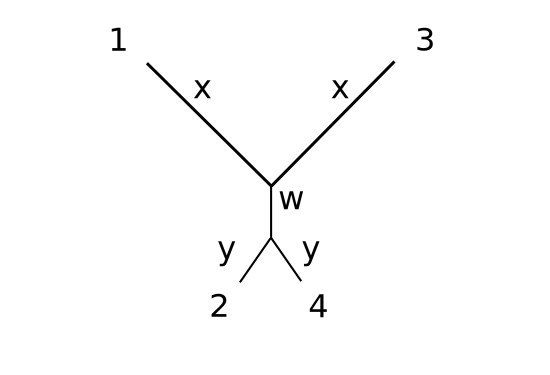
\includegraphics[width=.95\textwidth]{farris_blank}
\caption[short]{Farris topology $\tau_1$}
\end{subfigure}
\begin{subfigure}{.45\linewidth}
\centering
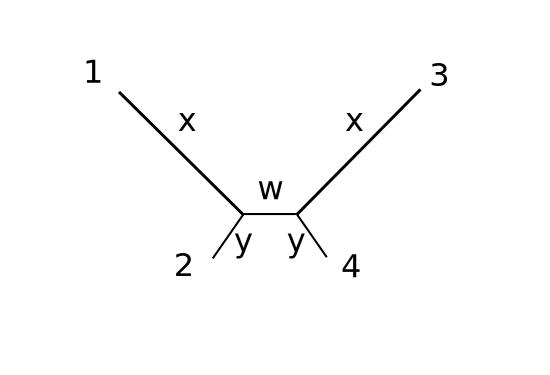
\includegraphics[width=.95\textwidth]{felsenstein_blank}
\caption[short]{Felsenstein topology $\tau_2$}
\end{subfigure}
\caption{Two simple topologies}
\end{figure}

Call $t=\{x,y,w\}$ and $t^*=\{x,y,y\}$, i.e., $t^*$ is the case where the bottom three branches all share the same parameter, the classical construction of this topology.
The branch length parameters are such that the probability of a change in character along the top two branches is $p_x=1-2x$, with corresponding equalities for the other two branches.
Here, $\{p_x,p_y,p_z\}\in[0,1/2]^3$ and $\{x,y,z\}\in[0,1]^3$.

\textbf{Justification for estimand:} It might be worth arguing why this form of the estimand $t$ is necessary.
I think the idea is that for either of these topologies, any maximum obtained will occur where the top two and bottom two branches are equal, though not necessarily the middle branch.
This would be good to show explicitly.

Table~\ref{tab:sitepatprob} contains calculations of site pattern frequencies under these two topologies, calculated using the Hadamard transform approach outlined in 8.6 of Semple and Steel \cite{semplesteel}.
Table~\ref{tab:likelihoods} contains calculations of likelihood values for fixed site patterns and topologies, with the maximum values over ancestral state patterns noted.

\begin{table}
\centering
\begin{tabular}{|l|l|l|}
\multicolumn{3}{c}{Classical}\\
    \hline
$s_j$   &$P(s_j|\tau_1,t^*)$&$P(s_j|\tau_2,t^*)$\\
    \hline
0000&$1+x^2+y^2+4xy^2+x^2y^2$&$1+2xy+2xy^2+x^2y+y^3+x^2y^2$\\
0001&$1+x^2-y^2-x^2y^2$&$1+x^2y-y^3-x^2y^2$\\
0010&$1-x^2+y^2-x^2y^2$&$1-x^2y+y^3-x^2y^2$\\
0100&$1+x^2-y^2-x^2y^2$&$1+x^2y-y^3-x^2y^2$\\
1000&$1-x^2+y^2-x^2y^2$&$1-x^2y+y^3-x^2y^2$\\
0011&$1-x^2-y^2+x^2y^2$&$1+2xy-2xy^2-x^2y-y^3+x^2y^2$\\
0101&$1+x^2+y^2-4xy^2+x^2y^2$&$1-2xy-2xy^2+x^2y+y^3+x^2y^2$\\
1001&$1-x^2-y^2+x^2y^2$&$1-2xy+2xy^2-x^2y-y^3+x^2y^2$\\
    \hline
\multicolumn{3}{c}{Modified}\\
    \hline
$s_j$   &$P(s_j|\tau_1,t)$&$P(s_j|\tau_2,t)$\\
    \hline
0000&$1+x^2+y^2+4xyw+x^2y^2$&$1+2xy+2xyw+x^2w+y^2w+x^2y^2$\\
0001&$1+x^2-y^2-x^2y^2$&$1+x^2w-y^2w-x^2y^2$\\
0010&$1-x^2+y^2-x^2y^2$&$1-x^2w+y^2w-x^2y^2$\\
0100&$1+x^2-y^2-x^2y^2$&$1+x^2w-y^2w-x^2y^2$\\
1000&$1-x^2+y^2-x^2y^2$&$1-x^2w+y^2w-x^2y^2$\\
0011&$1-x^2-y^2+x^2y^2$&$1+2xy-2xyw-x^2w-y^2w+x^2y^2$\\
0101&$1+x^2+y^2-4xyw+x^2y^2$&$1-2xy-2xyw+x^2w+y^2w+x^2y^2$\\
1001&$1-x^2-y^2+x^2y^2$&$1-2xy+2xyw-x^2w-y^2w+x^2y^2$\\
    \hline
\end{tabular}    
\caption{Site pattern probabilities.
All values are multiplied by $1/8$.}
\label{tab:sitepatprob}
\end{table}

\begin{table}
\centering
\begin{tabular}{|l|ll|}
\multicolumn{3}{c}{$P(z_j|s_j,\tau_1,t)$}\\
\hline
& \multicolumn{2}{|c|}{$z_j$}\\
    \hline
$s_j$    &00                              &01\\
    \hline
0000&$(1+x)^2   (1+w)(1+y)^{2*}$          &$(1+x)^2   (1-w)(1-y)^2$\\
0001&$(1+x)^2   (1+w)(1+y)(1-y)^*$        &$(1+x)^2   (1-w)(1+y)(1-y)$\\
0010&$(1+x)^2   (1+w)(1+y)(1-y)^*$        &$(1+x)^2   (1-w)(1+y)(1-y)$\\
0100&$(1+x)(1-x)(1+w)(1+y)^{2*}$          &$(1+x)(1-x)(1-w)(1-y)^2$\\
1000&$(1+x)(1-x)(1+w)(1+y)^{2*}$          &$(1+x)(1-x)(1-w)(1-y)^2$\\
0011&$(1+x)(1-x)(1+w)(1+y)(1-y)^{\dagger}$&$(1+x)(1-x)(1-w)(1+y)(1-y)$\\
0101&$(1+x)^2   (1+w)(1-y)^{2\ddagger}$   &$(1+x)^2   (1-w)(1+y)^{2\ddagger}$\\
1001&$(1+x)(1-x)(1+w)(1+y)(1-y)^{\dagger}$&$(1+x)(1-x)(1-w)(1+y)(1-y)$\\
    \hline
    \hline
&10                           &11\\
    \hline
0000&$(1-x)^2   (1-w)(1+y)^2$     &$(1-x)^2   (1+w)(1-y)^2$\\
0001&$(1-x)^2   (1-w)(1+y)(1-y)$  &$(1-x)^2   (1+w)(1+y)(1-y)$\\
0010&$(1-x)^2   (1-w)(1+y)(1-y)$  &$(1-x)^2   (1+w)(1+y)(1-y)$\\
0100&$(1+x)(1-x)(1-w)(1+y)^2$     &$(1+x)(1-x)(1+w)(1-y)^2$\\
1000&$(1+x)(1-x)(1-w)(1+y)^2$     &$(1+x)(1-x)(1+w)(1-y)^2$\\
0011&$(1+x)(1-x)(1-w)(1+y)(1-y)$  &$(1+x)(1-x)(1+w)(1+y)(1-y)^{\dagger}$\\
0101&$(1-x)^2   (1-w)(1-y)^2$     &$(1-x)^2   (1+w)(1+y)^{2\ddagger}$\\
1001&$(1+x)(1-x)(1-w)(1+y)(1-y)$  &$(1+x)(1-x)(1+w)(1+y)(1-y)^{\dagger}$\\
    \hline
    \multicolumn{3}{c}{$P(z_j|s_j,\tau_2,t)$}\\
\hline
& \multicolumn{2}{|c|}{$z_j$}\\
    \hline
$s_j$    &00                              &01\\
    \hline
0000&$(1+x)^2   (1+w)(1+y)^{2*}$           &$(1+x)(1-x)(1-w)(1+y)(1-y)$\\
0001&$(1+x)^2   (1+w)(1+y)(1-y)^{\ddagger}$&$(1+x)(1-x)(1-w)(1+y)^{2\ddagger}$\\
0010&$(1+x)(1-x)(1+w)(1+y)^{2\ddagger}$    &$(1+x)^2   (1-w)(1+y)(1-y)^{\ddagger}$\\
0100&$(1+x)^2   (1+w)(1+y)(1-y)^{\ddagger}$&$(1+x)(1-x)(1-w)(1-y)^2$\\
1000&$(1+x)(1-x)(1+w)(1+y)^{2\ddagger}$    &$(1-x)^2   (1-w)(1+y)(1-y)$\\
0011&$(1+x)(1-x)(1+w)(1+y)(1-y)^{\ddagger}$&$(1+x)^2   (1-w)(1+y)^{2\ddagger}$\\
0101&$(1+x)^2   (1+w)(1-y)^{2\ddagger}$    &$(1+x)(1-x)(1-w)(1+y)(1-y)^{\ddagger}$\\
1001&$(1+x)(1-x)(1+w)(1+y)(1-y)^{\ddagger}$&$(1-x)^2   (1-w)(1+y)^{2\ddagger}$\\
    \hline
    \hline
&10                           &11\\
    \hline
0000&$(1+x)(1-x)(1-w)(1+y)(1-y)$             &$(1-x)^2   (1+w)(1-y)^2$\\
0001&$(1+x)(1-x)(1-w)(1-y)^2$                &$(1-x)^2   (1+w)(1+y)(1-y)$\\
0010&$(1-x)^2   (1-w)(1+y)(1-y)$             &$(1+x)(1-x)(1+w)(1-y)^2$\\
0100&$(1+x)(1-x)(1-w)(1+y)^{2\ddagger}$      &$(1-x)^2   (1+w)(1+y)(1-y)$\\
1000&$(1+x)^2   (1-w)(1+y)(1-y)^{\ddagger}$  &$(1+x)(1-x)(1+w)(1-y)^2$\\
0011&$(1-x)^2   (1-w)(1-y)^2$                &$(1+x)(1-x)(1+w)(1+y)(1-y)^{\ddagger}$\\
0101&$(1+x)(1-x)(1-w)(1+y)(1-y)^{\ddagger}$  &$(1-x)^2   (1+w)(1+y)^{2\ddagger}$\\
1001&$(1+x)^2   (1-w)(1-y)^{2\ddagger}$      &$(1+x)(1-x)(1+w)(1+y)(1-y)^{\ddagger}$\\
\hline
\end{tabular}    
\caption{Likelihood calculations for all site patterns and internal states of Farris topology.
Maxima determined row-wise (i.e., by site pattern).
All values multiplied by $1/32$.
Key: $^*$ unique maximum value corresponding to unique internal state; $^\dagger$ unique maximum value corresponding to multiple internal states; $^\ddagger$ multiple maximum values corresponding to multiple internal states.}
\label{tab:likelihoods}
\end{table}

\subsection{Attempts to bound the likelihoods}

Ideally we could show for some generating parameters $t^*$ that there are simple bounds such that
$$
J(\tau', \hat{t}_1; \tau^*, t^*) \geq \underline{J}_1 > \overline{J}_2 \geq J(\tau^*, \hat{t}_2; \tau^*, t^*)
$$
where the fact that $\underline{J}_1 > \overline{J}_2$ will be obvious.
This approach could work since we have very particular forms for the prior probabilities and the likelihoods; we would need to find values of $t^*$ that minimize the probability (from the generating parameters) placed on those cases where the likelihood for the generating parameters is higher than those for a candidate parameter.
The frustrating aspect of this would be deriving a form for $J(\tau, \hat{t}; \tau^*, t^*)$ since it involves constrained maximization over three separate parameters: $x, y$ and $w$.

Since $x$ and $y$ are both in $[0,1]$ we have ready-made bounds available, though they may not be as tight as we want.
For example, in the case where both $x,y > 1/2$ we can compute upper and lower bounds on the generating probabilities by plugging in the appropriate value to Table~\ref{tab:sitepatprob}.

This is still ad hoc in that we need to fix an upper or lower bound for $x$ and $y$ to obtain these bounds.
Ideally we would seek tight bounds $(\underline{x}, \overline{x})$ and $(\underline{y}, \overline{y})$, where ``tight'' refers to how close they approximate the likelihoods they are bounding and not the parameters.

\subsection{Simplifying the likelihoods}

To simplify matters, we will first focus on bounding the the terms with the generating probabilities as they are more complicated.
Assume $\tau^*=\tau_1$ and $t^*=\{x,y,y\}$ so that
\begin{align}
\label{eq:information}
H_{\tau_1}(x, y;x', y', w') &= \sum_{j} P(s_j | \tau_1, \{x,y,y\}) \cdot \log P(s_j | \tau', \{x',y',w'\}) \nonumber \\ 
&:= \sum_{j} p(s_j) \cdot \log P(s_j | \tau', \{x',y',w'\}).
\end{align}
By Gibbs inequality,
$$
H_{\tau_1}(x, y;x', y', w') \le H_{\tau_1}(x, y;x, y, y),
$$
though this bound can be made tighter.
In our simplifications we will make use of the constants
$$
a = p(0100) + p(1000) + p(0011) + p(1001) = (4-2x^2-2y^2)/8,
$$
$$
b = p(1000) + p(0010) + p(0011) + p(1001) = (4-2x^2-2y^2)/8,
$$
$$
c = p(0001) + p(0010) + p(0100) + p(1000) = (4-4x^2y^2)/8
$$
and
$$
d = p(0101) + p(1001) = (2-4xy^2+2x^2y^2)/8
$$
with corresponding bounds
$$
0 \le a,b,c \le \frac{1}{2}
$$
and
$$
0 \le d \le \frac{1}{4}.
$$

Our key approach will be to decompose the likelihood as
\begin{equation}
\label{eq:partial-likelihood}
L^{(i)}(x', y', w') = H_{\tau_1}(x,y;x',y',w') + L^{p,(i)}(x',y',w')
\end{equation}
where the first term is \eqref{eq:information} and the second term will be a weighted sum of the $\log$s of values from Table~\ref{tab:likelihoods}, the superscript indicating which choices for ancestral state likelihood values we choose.
Define
$$
\{\hat{x}, \hat{y}, \hat{w}, \hat{i}\} = \arg\max_{\{x,y,w,i\}} \ L^{p,(i)}(x,y,w).
$$
We have upper and lower bounds for \eqref{eq:partial-likelihood} in the form
$$
H_{\tau_1}(x,y; \hat{x}, \hat{y}, \hat{w}) + L^{p,(\hat{i})}(\hat{x}, \hat{y}, \hat{w}) \le \max_{x,y,w} \ L^{(i)}(x,y,w) \le H(x,y;x,y,y) + L^{p,(\hat{i})}(\hat{x}, \hat{y}, \hat{w}).
$$

\textbf{Argument for lower bound}: This makes intuitive sense, though may be difficult to show in general.
Can we not just say $\max_u f(u) + g(u)$ is greater than $f(u') + g(u')$ for any $u'$ that doesn't maximize $f(u) + g(u)$ just by definition?
There could be multiple maxima, but that's why we have greater than or equal to.
I think the only thing we'd need to show is that a maximum exists, but since $\{x,y,w\}$ are supported on a closed set this is certainly true.
I must be missing something.

\textbf{Argument for upper bound}: I think this is true mostly because $\max_u f(u) + g(u)$ should be less than $\max_u f(u) + \max_u g(u)$ by some triangle inequality argument.
If we were to actually maximize the full likelihood, we should get something smaller than maximizing some form of it that we consider by looking at the parts separately.
For a fixed $\{x^*, y^*\}$ we can calculate this upper bound directly---can we obtain it as a useful-looking function of these parameters in the general case?

\subsubsection{A simplified Farris likelihood}

The likelihood for the Farris topology is less complicated than that of the Felsenstein since only one site pattern has an ambiguous likelihood---all site patterns except \texttt{0101} have a fixed value for their likelihood when taking the maximum.
To fix this value, we will consider an upper bound on the partial likelihood by setting the value for site pattern 0011 to $(1+x)^2(1+w)(1+y)^2$.
Here the partial likelihood $L_{fa}^{p,(i)}(x,y,w)$ takes the form:
$$
L_{fa}^{p} = (2-a)\log(1+x)+a\log(1-x)+(2-b)\log(1+y)+b\log(1-y)+\log(1+w),
$$
and this has a maximum
$$
\hat{L}_{fa}^{p} = (2-a)\log(2-a)+a\log(a)+(2-b)\log(2-b)+b\log(b)+\log(2).
$$

\subsubsection{A simplified Felsenstein likelihood}

We construct similar bounds on the Felsenstein likelihood, though to make matters simpler we replace all $(1+y)$ terms in Table~\ref{tab:likelihoods} with $(1-y)$ to obtain a lower bound.
Unlike the Farris partial likelihood, the likelihood in this case has one of six forms:
$$
L_{fe}^{(1)} = 2\log(1+x)+(2-c-2d)\log(1+y)+(c+2d)\log(1-y)+\log(1-w),
$$
$$
L_{fe}^{(2)} = (2-c-2d)\log(1+x)+(c+2d)\log(1-x)+2\log(1+y)+\log(1-w),
$$
$$
L_{fe}^{(3)} = (2-2d)\log(1+x)+2d\log(1-x)+(2-c)\log(1+y)+c\log(1-y)+\log(1-w),
$$
$$
L_{fe}^{(4)} = (2-c)\log(1+x)+c\log(1-x)+(2-2d)\log(1+y)+2d\log(1-y)+\log(1-w),
$$
$$
L_{fe}^{(5)} = (2-d)\log(1+x)+d\log(1-x)+(2-c-d)\log(1+y)+(c+d)\log(1-y)+\log(1-w)
$$
and
$$
L_{fe}^{(6)} = (2-c-d)\log(1+x)+(c+d)\log(1-x)+(2-d)\log(1+y)+d\log(1-y)+\log(1-w)
$$
with maxima
$$
\hat{L}_{fe}^{(1)} = \hat{L}_{fe}^{(2)} = 2\log(2)+(2-c-2d)\log(2-c-2d)+(c+2d)\log(c+2d)
$$
$$
\hat{L}_{fe}^{(3)} = \hat{L}_{fe}^{(4)} = (2-2d)\log(2-2d)+2d\log(2d)+(2-c)\log(2-c)+c\log(c)
$$
and
$$
\hat{L}_{fe}^{(5)} = \hat{L}_{fe}^{(6)} = (2-d)\log(2-d)+d\log(d)+(2-c-d)\log(2-c-d)+(c+d)\log(c+d).
$$

\textbf{TODO}: cases for $\{x, y\}$ where each of the above is the corresponding maximum.
I think the first is always greater than or equal to the other two, but I haven't been able to show it yet.
It may take a little information theory--fu, or just standard application of the bounds in the introduction to this section.

\paragraph{Example}

Set $\{x, y\} = \{0.25, 0.25\}$.
For a Farris zone generating topology, we have
$$
a = b = 0.46875
$$
resulting in
$$
\hat{L}_{fa}^{p}(\hat{x}, \hat{y}, \hat{w}) \approx -2.17803560694
$$
and
$$
H_{fa}(x,y;x,y,y) \approx -2.07509999739.
$$
Computing the upper bound yields
$$
\max_{x,y,w} \ L_{fa}(x,y,w) \le -4.25313560433
$$
and it remains to show that 
$$
\max_{x,y,w} \ L_{fe}(x,y,w) \ge -4.25313560433
$$

For the same generating parameters,
$$
c = 0.498046875, \ d = 0.2431640625,
$$
resulting in
$$
\hat{L}_{fe}(\hat{x}, \hat{y}, \hat{w}) \approx -2.07919739112
$$
Calculating shows%
    %
    \footnote{It's not a typo that $\hat{L}_{fe}$ and $H_{fe}(x,y; \hat{x}, \hat{y}, \hat{w})$ are the same---at least not in the code.
        I should try to show why this is the case.
        }
    %
$$
H_{fe}(x,y; \hat{x}, \hat{y}, \hat{w}) \approx -2.07919739112
$$
and
$$
\max_{x,y,w} \ L_{fe}(x,y,w) \ge -4.15839478224 > -4.25313560433 \ge \max_{x,y,w} \ L_{fa}(x,y,w)
$$
where site patterns are generated from the Farris zone topology.
Confirming, run \texttt{python}'s numerical optimization solver for $\{.25, .25\}$.
Since we are computing a constrained maximization, we can find a global maximum using basin hopping, and doing so yields
$$
\max_{x,y,w} \ L_{fa}(x,y,w) \approx -4.5101771294218045
$$
and
$$
\max_{x,y,w} \ L_{fe}(x,y,w) \approx -4.1544859851260281.
$$
Woohoo!

\paragraph{General example}

We want to find values for $\{x,y\}$ where
$$
H_{fe}(x,y; 1, 0, 1-c-2d) + \hat{L}_{fe}(c,d) \ge H_{fa}(x,y; x, y, y) + \hat{L}_{fa}(a,b).
$$
We can cheat a bit and plot the values at which this is true.
This may give us some insight into what form these regions of inconsistency take---see Fig.~\ref{fig:inconsistency-farris}.

\begin{figure}
\centering
\includegraphics[width=.9\textwidth]{ineqs-max-far-gen}
\caption{Regions of inconsistency}
\label{fig:inconsistency-farris}
\end{figure}

%%%%%%%%%%%%%%%%%%%%%%%%%%%%%%%%%%%%%%%%%%%%%%%%%%%%%%%%%%%%%%%%%%%%%%%%%%%%%%%%%%%%%%%%%%%%%%%%%%%%%%%
\newpage

\section{Temporarily unused text I may want later to show more general results on the likelihood estimates}

Some scratch work:
$$
a = b = (4-2x^2-2y^2)/8,
$$
$$
c+2d = 1-xy^2, \ 2-c-2d = 1+xy^2
$$
$$
H_{fe}(x,y; 1, 0, 1-c-2d) \propto (2-4xy^2+2x^2y^2)\log(1-2xy^2+x^2y^4) + (2+4xy^2+2x^2y^2)\log(1+2xy^2+x^2y^4)+(4-4x^2y^2)\log(1-x^2y^4)
$$
$$
H_{fa}(x,y; x, y, y) \propto (2-4xy^2+2x^2y^2)\log(1-2xy^2+x^2y^4) + (2+4xy^2+2x^2y^2)\log(1+2xy^2+x^2y^4)+(4-4x^2y^2)\log(1-x^2y^4)
$$
$$
\hat{L}_{fe} \propto 2\log(2) + (1+xy^2)\log(1+xy^2) + (1-xy^2)\log(1-xy^2)
$$
$$
\hat{L}_{fa} \propto \log(2) + (4-2a)\log(2-a)+2a\log(a).
$$


\subsubsection{A counterexample in branch lengths}

Let $(\tau^*, t^*)=(\tau_1, \{x,y,x\})$.
We claim there exist $\{x,y\}$ and $\{x, \tilde{y}\}$ such that
$$
L'(\tau^*, t^*; \tau^*, \{x, \tilde{y}\}) > L'(\tau^*, t^*; \tau^*, t^*).
$$
The model is given by values in the Table.
Set $x=0$ to obtain
$$
L'(\tau^*, t^*; \tau^*, t^*) \propto 8\log(1+y)
$$
and
$$
L'(\tau^*, t^*; \tau^*, \{0, \tilde{y}\}) \propto 8\log(1+\tilde{y}).
$$
Therefore, if $\tilde{y} > y$ we have an inconsistency.

\begin{table}
\centering
\begin{tabular}{|l|l|l|}
    \hline
$s_j$   &$P(s_j|\tau_1,t)$&$\max_{z_j} \ P(s_j,z_j|\tau_1,t)$\\
    \hline
0000&$1+2x^2+4x^2y+x^4$&$(1+x)^4(1+y)$\\
0001&$1-x^4$&$(1+x)^3(1+y)(1-x)$\\
0010&$1-x^4$&$(1+x)^3(1+y)(1-x)$\\
0100&$1-x^4$&$(1+x)^3(1+y)(1-x)$\\
1000&$1-x^4$&$(1+x)^3(1+y)(1-x)$\\
0011&$1+2x^2-4x^2y+x^4$&max$\{(1+x)^2(1+y)(1-x)^2,(1+x)^4(1-y)\}$\\
0101&$1-2x^2+x^4$&$(1+x)^2(1+y)(1-x)^2$\\
1001&$1-2x^2+x^4$&$(1+x)^2(1+y)(1-x)^2$\\
    \hline
\end{tabular}    
\caption{Counterexample 1.}
\label{tab:sitepatprob_case1}
\end{table}

\subsubsection{A counterexample in topologies}

Let $(\tau^*, t^*)=(\tau_1, \{x,y,y\})$.
We claim there exist $\{x,y\}$ such that
$$
L'(\tau^*, t^*; \tau_2, t^*) > L'(\tau^*, t^*; \tau^*, t^*).
$$
Set $y=0$ to obtain parameters given in Table.
We have
$$
L'(\tau^*, t^*; \tau^*, t^*) \propto 4(1+x^2)\log(1+x^2)+4(1-x^2)\log(1-x^2)+4(1+x^2)\log((1+x)^2)+4(1-x^2)\log((1+x)(1-x))
$$
and
$$
L'(\tau^*, t^*; \tau_2, t^*) \propto 3(1+x^2)\log((1+x)^2)+3(1-x^2)\log((1+x)^2)+(1+x^2)\log((1+x)(1-x))+(1-x^2)\log((1+x)(1-x)).
$$
The difference being greater than zero, i.e.,
$$
L'(\tau^*, t^*; \tau_2, t^*) - L'(\tau^*, t^*; \tau^*, t^*) > 0,
$$
simplifies to
$$
4x^2(\log(1-x^2)-\log(1+x^2)+\log(1-x)-\log(1+x)) - 2(2\log(1+x^2)+2\log(1-x^2)-\log(1+x)+\log(1-x)) > 0.
$$
Let $0 < x < 1/\sqrt{2}$ so that the above inequality becomes
$$
-\log(1-x^2)-3\log(1+x^2) > 0
$$
or
$$
(1+x^2)^3(1-x^2) < 1.
$$
Applying $x<1/\sqrt{2}$ shows if
$$
x < \sqrt{-1+2^{1/3}} \approx 0.5098
$$
we have an inconsistency.

\begin{table}
\centering
\begin{tabular}{|l|l|l||l|l|}
    \hline
$s_j$   &$P(s_j|\tau_1,t)$&$\max_{z_j} \ P(s_j,z_j|\tau_1,t)$&$P(s_j|\tau_2,t)$&$\max_{z_j} \ P(s_j,z_j|\tau_2,t)$\\
    \hline
0000&    $1+x^2$ & $(1+x)^2$ & 1 & $(1+x)^2$\\
0001&    $1+x^2$ & $(1+x)^2$ & 1 & $(1+x)^2$\\
0010&    $1+x^2$ & $(1+x)^2$ & 1 & $(1+x)^2$\\
0100&    $1-x^2$ & $(1+x)(1-x)$ & 1 & $(1+x)^2$\\
1000&    $1-x^2$ & $(1+x)(1-x)$ & 1 & $(1+x)^2$\\
0011&    $1+x^2$ & $(1+x)^2$ & 1 & $(1+x)(1-x)$\\
0101&    $1-x^2$ & $(1+x)(1-x)$ & 1 & $(1+x)^2$\\
1001&    $1-x^2$ & $(1+x)(1-x)$ & 1 & $(1+x)(1-x)$\\
    \hline
\end{tabular}    
\caption{Counterexample 2.}
\label{tab:sitepatprob_case2}
\end{table}

\subsubsection{More fleshed out counterexamples}

The above counterexamples are highly pathological, but they show there exist whole spaces of parameters yielding inconsistencies.
It seems as long as $x$ and $y$ are ``small enough'' we see inconsistency.

\subsection{start}

We can calculate the probability of a particular site pattern under this topology from the probability that all character states are equal as
$$
P(0000|\tau^*,t) = \frac{1}{8}(1+x^2+z^2+4xyz+x^2z^2)
$$
where the probability of any site pattern will be the same as above with the corresponding branch length parameter replaced with its negative.
For example, if we have the pattern $0001$, since the last branch has length $z$ we replace it with $-z$ and obtain
$$
P(0001|\tau^*,t) = \frac{1}{8}(1+x^2-z^2-x^2z^2).
$$
All possible site pattern probabilities are given in Table~\ref{tab:sitepatprob}.
All likelihoods and their maximal values are given in Table~\ref{tab:likelihoods}.

It can be shown (I'll do it later) that for our $t^*$ the right-hand term above is $-16\log 8$.
Moreover, for $t=\{x,y,z\}$
\begin{equation}
\sum_{s} \log P(s | \tau^*, t) + \log P(\xi | s, \tau^*, t) = -16\log 8 + f(x,y,z) + g(x,y,z)
\end{equation}
where
\begin{align}
f(x,y,z) &= 4\log(1+x)+4\log(1-x)+4\log(1+z)+4\log(1-z)+\\
& 3\log(1+x^2)+3\log(1+z^2)+\\
& \log((1+x^2)(1+z^2)+4xyz) + \log((1+x^2)(1+z^2)-4xyz).
\end{align}
and
\begin{align}
g(x,y,z) &= 10\log(1+x)+10\log(1+z)+4\log(1-x)+4\log(1-z)+7\log(1+y)+\\
& \left\{ 
  \begin{array}{l}
  2\log(1+x)+2\log(1-z)+\log(1+y)\\
  2\log(1+x)+2\log(1+z)+\log(1-y)\\
  2\log(1-x)+2\log(1-z)+\log(1+y)\\
  \end{array} \right.
\end{align}
whose component will be chosen based on whichever yields the maximum value for $\log L''$.

\subsection{Two fixed topologies}

\subsection{Special case: $x=z=0$}

Consider now setting all data-generating branch length parameters $t^*$ to zero; this yields equal probabilities of $1/8$ for each site pattern.
By the inequality of Gibbs we have
$$
\sum_{s} P(s|\tau^*,t^*)\log P(s|\tau^*,t^*) \geq \sum_{s} P(s|\tau^*,t^*)\log P(s|\tau^*,t)
$$
summing over all site patterns, which is equivalent to
$$
\sum_{s} \log P(s|\tau^*,t^*) \geq \sum_{s} \log P(s|\tau^*,t).
$$
We must show, then, that there exist $t\neq t^*$ such that
$$
\max_{\xi_s} \ \sum_{s} \log P(s | \tau^*, t) + \log P(\xi_s | s, \tau^*, t) > \max_{\xi_s} \sum_{s} \log P(s | \tau^*, t^*) + \log P(\xi_s | s, \tau^*, t^*).
$$
Assume for $t$ that $x=z=0$ but $y\neq 0$.
Clearly site pattern probabilities are still all equal, and the first summand of each side of the inequality can be ignored in this case.
Call
$$
f(x,y,z) = \sum_{s} \log P(\xi_s | s, \tau^*, t=\{x,y,z\}).
$$
For branch lengths $\{x,y,z\}$, by considering all eight cases (see Table~\ref{tab:likelihoods}) of site patterns we can show that in terms of branch length \emph{probabilities}%
	%
    \footnote{The function $f$ has inverse $f^{-1}(u)=(1-u)/2$ so that the probability of a change along a branch of length $x$ maps to $(1-x)/2$ and the probability of no change maps to $(1+x)/2$.}
    %
\begin{align}
f(x,y,z) \propto & \ 10\log(1+x)+10\log(1+z)+4\log(1-x)+4\log(1-z)+7\log(1+y)+\\
& \left\{ 
  \begin{array}{l}
  2\log(1+x)+2\log(1-z)+\log(1+y)\\
  2\log(1+x)+2\log(1+z)+\log(1-y)\\
  2\log(1-x)+2\log(1-z)+\log(1+y)\\
  \end{array} \right.
\end{align}
whose last summand will be chosen based on whichever yields the maximum value and where the proportionality is due to requiring branch length parameters $\{x,y,z\}$ to be multiplied by $1/2$ to map them to probabilities.
We see that
$$
f(x,y,z)|_{x=z=0} = 8\log(1+y)
$$
and thus require the constraint
$$
8\log(1+y) > 0
$$
or that $y$ is any value bounded away from zero, and will obtain a maximum at $y=1$ or $p_y=0$.

\subsection{Special case: $x=z\neq 0$}


Fixing $x=z=0$ is a little too pathological---anything can happen when we're flipping coins to determine terminal characters.
Let's investigate a relaxed yet still special case where branches to the tips are all equal but allowed to be nonzero.
So we set $\tau^*=\tau$, $t^*=\{x,x,y\}$ and $t=\{x,x,\tilde{y}\}$ where the same terminal branches are used for both parameter sets with only the internal branch different.
Removing terms involving only $x$ and redundant $y$ shows that we need only concern ourselves with the objective functions
\begin{align*}
L_1(u) =& 8\log(1+u) + \\
  &(1+2x^2+4x^2y+x^4)\log(1+2x^2+4x^2u+x^4) + \\
  &(1+2x^2-4x^2y+x^4)\log(1+2x^2-4x^2u+x^4)
\end{align*}
if $(1+u)(1-x)^2 > (1-u)(1+x)^2$---or, more simply, if $u > 2x / (1+x^2)$---and
\begin{align*}
L_2(u) =& (7-2x^2+4x^2y-x^4)\log(1+u) + \\
  &(1+2x^2-4x^2y+x^4)\log(1-u) + \\
  &(1+2x^2+4x^2y+x^4)\log(1+2x^2+4x^2u+x^4) + \\
  &(1+2x^2-4x^2y+x^4)\log(1+2x^2-4x^2u+x^4)
\end{align*}
otherwise.
We can rule out the case where $\tilde{y} < y$ in $L_1$ by the inequality of Gibbs and using a similar argument along with the inequality
$$
1+2x^2-4x^2y+x^4 \le 7-2x^2+4x^2y-x^4
$$
implies we can rule out $\tilde{y} < y$ in $L_2$ as well (actually I'm not sure if I believe this anymore; the case of $L_1$ definitely holds, though).
This leaves us with four sets of inequalities where an inconsistency will arise,
$$
\left\{\tilde{y} > y > \frac{2x}{1+x^2}, \ L_1(\tilde{y}) > L_1(y)\right\}, 
$$
$$
\left\{\tilde{y} > \frac{2x}{1+x^2} > y, \ L_1(\tilde{y}) > L_2(y)\right\}, 
$$
$$
\left\{\frac{2x}{1+x^2} > \tilde{y} > y, \ L_2(\tilde{y}) > L_2(y)\right\},
$$
and
$$
\left\{\frac{2x}{1+x^2} > y > \tilde{y}, \ L_2(\tilde{y}) > L_2(y)\right\}.
$$
Simplifying shows
$$
L_2(u) = L_1(u) + (1+2x^2-4x^2y+x^4)\log\frac{1-u}{1+u} \le L_1(u).
$$
Can we use this fact?
I believe in my heart of hearts, perhaps foolishly, that the first set of inequalities holds categorically.
The fact above will then imply the second set of inequalities must also hold.
The tricky bits are the last two sets of inequalities.

If you'll allow me to indulge in a bit of cheating, I provide a few plots showing---for fixed $x$---the regions where inconsistencies arise.
It looks like there is some regularity that we must be able to exploit somehow, if only to show that for a fixed $x$ there are inequalities in $y$ and $\tilde{y}$ governing consistency.

%\begin{figure}
%\centering
%\includegraphics[width=.3\textwidth]{ineqs-x-0_25}\hfill
%\includegraphics[width=.3\textwidth]{ineqs-x-0_75}\hfill
%\includegraphics[width=.3\textwidth]{ineqs-x-0_9}
%\caption{Various regions of inconsistency for fixed $x$}
%\end{figure}

Say $\tau_1$ is the ``Felsenstein zone'' tree and $\tau_2$ is the ``Farris zone'' tree, but both trees have a different value for its middle, connecting branch.
%EM widdershins!! This still depends on how we draw them, no?
The tips are labeled widdershins proceeding from the top-left tip.
\begin{verbatim}
Felsenstein:
1\      /3
   >--< 
2/      \4

Farris:
1\ /3
  | 
2/ \4
\end{verbatim}
Our branch length parameters $t=\{x,y,z\}$ will consist of transformed probabilities where $y$ corresponds to this middle branch.
For $p_x\in[0,1/2]$ defined as
$$p_x = Pr(\mbox{change occurred along branch})$$
then $x = 1-2p_x$.
The parameter $x$ takes values in $[0,1]$ and will appear in likelihood calculations as either $(1+x)$ or $(1-x)$.
Properties for $y$ and $z$ are identical.
Assume for the moment that $\tau^*=\tau_1$ and $t^*=\{x,y,z\}$.

\subsubsection{Example site pattern: \texttt{0101}}

It can be shown that the only $A$ for which there is more than one partition for $\tau_2$ is for the site pattern \texttt{0101}.
In this case
$$A_1(\tau_1) = \{(1+x)^2(1-z)^2 = (1-x)^2(1+z)^2\},$$
$$A_2(\tau_1) = \{(1+x)(1+y)(1-z) = (1-x)(1-y)(1+z)\},$$
$$A_3(\tau_1) = \{(1-x)(1+y)(1+z) = (1+x)(1-y)(1-z)\}$$
and
$$A_1(\tau_2) = \{(1-z)^2(1+y) = (1+z)^2(1-y)\},$$
$$A_2(\tau_2) = \{(1-z)^2(1+x)^2 = (1+z)^2(1-x)^2\},$$
$$A_3(\tau_2) = \{(1+x)^2(1-y) = (1-x)^2(1+y)\}.$$

Now, the probability of generating this site pattern under $\tau^*$ is given as
$$
Pr(\texttt{0101} | \tau^*, t^*) = \frac{1}{8}(1-2xz+y(x^2+z^2-2xz)+x^2z^2).
$$

\subsubsection{Example site pattern: \texttt{0000}}

In the case of site pattern \texttt{0000} the refinements $A$ for both topologies are single-element partitions.
In other words, no configuration of branch lengths will result in an ancestral state other than \texttt{00}.
Here we have the probability
$$
Pr(\texttt{0000} | \tau^*, t^*) = \frac{1}{8}(1+2xz+y(x^2+z^2+2xz)+x^2z^2)
$$
and the maximum value for $Pr(\xi | \texttt{0000}, \tau, t^*)$ for both $\tau_1$ and $\tau_2$ is
$$
Pr(\xi | \texttt{0000}, \tau, t^*) = (1+x)^2(1+z)^2(1+y).
$$

\subsubsection{All refinements with multi-element partitions}

(show calculations for all refinements that have multiple partitions)

\subsection{Numerical sanity check}

Let's suppose site pattern \texttt{0101} is the only one that drives some disconcert between the generating tree and the maximum likelihood tree.
For a number of combinations of $\{x,y,z\}$ we need to calculate first
$$
Pr(\texttt{0101} | \tau^*, t^*) = \frac{1}{8}(1-2xz+y(x^2+z^2-2xz)+x^2z^2)
$$
and the maximum value over each $A_i(\tau)$ of $Pr(\xi | \texttt{0101}, \tau, t^*)$ for $\tau\in\{\tau_1, \tau_2\}$.
In other words, say we have the triplet $\{x,y,z\}=\{0.8,0.5,0.8\}$.
Then we have
$$
\max_{\xi} Pr(\xi | \texttt{0101}, \tau_1, t^*) = 0.0243, \ \max_{\xi} Pr(\xi | \texttt{0101}, \tau_2, t^*) = 0.6561, \ Pr(\texttt{0101} | \tau^*, t^*) = 0.0162.
$$
This doesn't yet tell us anything, as the probabilities for other site patterns may overwhelm this particular one, but gives a general flavor of how these computations will be performed.
Moreover, a different triplet of $\{x,y,z\}$ could obtain a different maximum value for $Pr(\xi | s, \tau, t^*)$.
This can be seen with the pattern \texttt{0011} where
$$
\max_{\xi} Pr(\xi | \texttt{0011}, \tau_1, t^*) = 0.6561, \ \max_{\xi} Pr(\xi | \texttt{0011}, \tau_2, t^*) = 0.0243, \ Pr(\texttt{0011} | \tau^*, t^*) = 0.1762
$$
meaning that if all else were equal---i.e., $\max_{\xi} Pr(\xi | s, \tau, t^*)$ were the same for $\tau_1$ and $\tau_2$ for all $s$---and that the maximum value actually occurs at this particular triplet $\{x,y,z\}$ then
$$
L(\tau_1) = 0.928 > 0.119 = L(\tau_2)
$$
and we have no contradiction.
That's a lot of ``if'' statements, so let's investigate in a little more generality.

\subsection{Differing branch lengths}

First, we do not wish to assume $\{x,y,z\}$ are the same for both trees.

\subsubsection{General case}

The generating probability $Pr(s | \tau^*, t^*)$ has a specific form given a Hadamard transformation of the branch length parameters, while the term proportional to $Pr(\xi | s, \tau, t^*)$ relies on taking the maximum over a function with multiple components.
All of this is easy to write into a computer program, and we can numerically find the maximum value over $\{\theta_1, \ldots, \theta_5\}\in[0,1]$ of each $L(\tau_1)$ and $L(\tau_2)$.
If $L(\tau_1) < L(\tau_2)$ we see that jointly maximizing branch lengths and ancestral states results in a contradiction.

In sufficient enough generality, we would look for any combination of $\{\tau_1,\tau_2\}$ that would result in this contradiction, but let's first focus on the two from the previous section.

\subsubsection{Classic formulations of topologies}

\begin{table}
\centering
\begin{tabular}{|l|l|}
    \hline
s   &$P(s)$\\
    \hline
0000&$1+x^2+y^2+4xy^2+x^2y^2$\\
0001&$1+x^2-y^2-x^2y^2$\\
0010&$1+x^2-y^2-x^2y^2$\\
0100&$1-x^2+y^2-x^2y^2$\\
1000&$1-x^2+y^2-x^2y^2$\\
0011&$1+x^2+y^2-4xy^2+x^2y^2$\\
0101&$1-x^2-y^2+x^2y^2$\\
1001&$1-x^2-y^2+x^2y^2$\\
    \hline
\end{tabular}    
\caption{Site pattern probabilities for Farris zone topology.
All values are multiplied by $1/8$.}
\end{table}

\begin{table}
\centering
\begin{tabular}{|l|l|}
    \hline
s   &$P(s)$\\
    \hline
0000&$1+2xy+2xy^2+x^2y+y^3+x^2y^2$\\
0001&$1+x^2y-y^3-x^2y^2$\\
0010&$1-x^2y+y^3-x^2y^2$\\
0100&$1+x^2y-y^3-x^2y^2$\\
1000&$1-x^2y+y^3-x^2y^2$\\
0011&$1+2xy-2xy^2-x^2y-y^3+x^2y^2$\\
0101&$1-2xy-2xy^2+x^2y+y^3+x^2y^2$\\
1001&$1-2xy+2xy^2-x^2y-y^3+x^2y^2$\\
    \hline
\end{tabular}    
\caption{Site pattern probabilities for Felsenstein zone topology.
All values are multiplied by $1/8$.}
\label{tab:sitepatprob-fels}
\end{table}

\begin{table}
\centering
\begin{tabular}{|l|ll|}
    \hline
    &00                              &01\\
    \hline
0000&$(1+x)^2(1+y)^{3*}$          &$(1+x)^2(1-y)^3$\\
0001&$(1+x)^2(1+y)^2(1-y)^*$       &$(1+x)^2(1+y)(1-y)^2$\\
0010&$(1+x)^2(1+y)^2(1-y)^*$       &$(1+x)^2(1+y)(1-y)^2$\\
0100&$(1+x)(1-x)(1+y)^{3*}$       &$(1+x)(1-x)(1-y)^3$\\
1000&$(1+x)(1-x)(1+y)^{3*}$       &$(1+x)(1-x)(1-y)^3$\\
0011&$(1+x)^2(1+y)(1-y)^{2}$          &$(1+x)^2(1-y)(1+y)^{2\ddagger}$\\
0101&$(1+x)(1-x)(1+y)^2(1-y)^{\dagger}$    &$(1+x)(1-x)(1+y)(1-y)^2$\\
1001&$(1+x)(1-x)(1+y)^2(1-y)^{\dagger}$    &$(1+x)(1-x)(1+y)(1-y)^2$\\
    \hline
    \hline
&10                           &11\\
    \hline
0000&$(1-x)^2(1+y)^2(1-y)$        &$(1-x)^2(1+y)(1-y)^2$\\
0001&$(1-x)^2(1+y)(1-y)^2$     &$(1-x)^2(1+y)^2(1-y)$\\
0010&$(1-x)^2(1+y)(1-y)^2$     &$(1-x)^2(1+y)^2(1-y)$\\
0100&$(1+x)(1-x)(1+y)^2(1-y)$     &$(1+x)(1-x)(1+y)(1-y)^2$\\
1000&$(1+x)(1-x)(1+y)^2(1-y)$     &$(1+x)(1-x)(1+y)(1-y)^2$\\
0011&$(1-x)^2(1-y)^3$       &$(1-x)^2(1+y)^{3\ddagger}$\\
0101&$(1+x)(1-x)(1+y)(1-y)^2$  &$(1+x)(1-x)(1+y)^2(1-y)^{\dagger}$\\
1001&$(1+x)(1-x)(1+y)(1-y)^2$  &$(1+x)(1-x)(1+y)^2(1-y)^{\dagger}$\\
    \hline
\end{tabular}    
\caption{Likelihood calculations for all site patterns and internal states of Farris topology.
Maxima determined row-wise (i.e., by site pattern).
Key: $^*$ unique maximum value corresponding to unique internal state; $^\dagger$ unique maximum value corresponding to multiple internal states; $^\ddagger$ multiple maximum values corresponding to multiple internal states.}
\end{table}

\begin{table}
\centering
\begin{tabular}{|l|ll|}
    \hline
    &00                              &01\\
    \hline
0000&$(1+x)^2(1+y)^{3*}$          &$(1+x)(1-x)(1+y)(1-y)^2$\\
0001&$(1+x)^2(1+y)^2(1-y)^{*}$       &$(1+x)(1-x)(1+y)^2(1-y)$\\
0010&$(1+x)(1-x)(1+y)^{3\ddagger}$       &$(1+x)^2(1+y)(1-y)^{2\ddagger}$\\
0100&$(1+x)^2(1+y)^2(1-y)^*$       &$(1+x)(1-x)(1-y)^3$\\
1000&$(1+x)(1-x)(1+y)^{3\ddagger}$       &$(1-x)^2(1+y)(1-y)^2$\\
0011&$(1+x)(1-x)(1+y)^2(1-y)^{\dagger}$          &$(1+x)^2(1+y)^2(1-y)$\\
0101&$(1+x)^2(1+y)(1-y)^{2\ddagger}$    &$(1+x)(1-x)(1+y)(1-y)^2$\\
1001&$(1+x)(1-x)(1+y)^2(1-y)^{\dagger}$    &$(1+x)(1-x)(1+y)(1-y)^2$\\
    \hline
    \hline
&10                           &11\\
    \hline
0000&$(1+x)(1-x)(1+y)(1-y)^2$        &$(1-x)^2(1+y)(1-y)^2$\\
0001&$(1+x)(1-x)(1-y)^3$     &$(1-x)^2(1+y)^2(1-y)$\\
0010&$(1-x)^2(1+y)(1-y)^2$     &$(1+x)(1-x)(1+y)(1-y)^2$\\
0100&$(1+x)(1-x)(1+y)^2(1-y)^{\ddagger}$     &$(1-x)^2(1+y)^2(1-y)$\\
1000&$(1+x)^2(1+y)(1-y)^{2\ddagger}$     &$(1+x)(1-x)(1+y)(1-y)^2$\\
0011&$(1-x)^2(1-y)^3$       &$(1+x)(1-x)(1+y)^2(1-y)^{\dagger}$\\
0101&$(1+x)(1-x)(1+y)(1-y)^2$  &$(1-x)^2(1+y)^{3\ddagger}$\\
1001&$(1+x)(1-x)(1+y)(1-y)^2$  &$(1+x)(1-x)(1+y)^2(1-y)^{\dagger}$\\
    \hline
\end{tabular}    
\caption{Likelihood calculations for all site patterns and internal states of Felsenstein topology.
Maxima determined row-wise (i.e., by site pattern).
Key: $^*$ unique maximum value corresponding to unique internal state; $^\dagger$ unique maximum value corresponding to multiple internal states; $^\ddagger$ multiple maximum values corresponding to multiple internal states.}
\label{tab:likelihoods-fels}
\end{table}


\begin{table}
\centering
\begin{tabular}{|l|l|}
    \hline
s   &$P(s)$\\
    \hline
0000&$1+x^2+z^2+2xyz+x^2y+z^2y+x^2z^2$\\
0001&$1+x^2-z^2+x^2y-z^2y-x^2z^2$\\
0010&$1-x^2+z^2-x^2y+z^2y-x^2z^2$\\
0100&$1+x^2-z^2+x^2y-z^2y-x^2z^2$\\
1000&$1-x^2+z^2-x^2y+z^2y-x^2z^2$\\
0011&$1-x^2-z^2-2xyz-x^2y-z^2y+x^2z^2$\\
0101&$1+x^2+z^2-2xyz+x^2y+z^2y+x^2z^2$\\
1001&$1-x^2-z^2-2xyz-x^2y-z^2y+x^2z^2$\\
    \hline
\end{tabular}    
\caption{Site pattern probabilities for Felsenstein zone topology.
All values are multiplied by $1/8$.}
\label{tab:sitepatprob-fels}
\end{table}

\begin{table}
\centering
\begin{tabular}{|l|ll|}
    \hline
    &00                              &01\\
    \hline
0000&$(1+x)^2(1+y)(1+z)^{2*}$          &$(1+x)(1-x)(1-y)(1+z)(1-z)$\\
0001&$(1+x)^2(1+y)(1+z)(1-z)^{\ddagger}$       &$(1+x)(1-x)(1-y)(1+z)^{2\ddagger}$\\
0010&$(1+x)(1-x)(1+y)(1+z)^{2\ddagger}$       &$(1+x)^2(1-y)(1+z)(1-z)^{\ddagger}$\\
0100&$(1+x)^2(1+y)(1+z)(1-z)^{\ddagger}$       &$(1+x)(1-x)(1-y)(1-z)^2$\\
1000&$(1+x)(1-x)(1+y)(1+z)^{2\ddagger}$       &$(1-x)^2(1-y)(1+z)(1-z)$\\
0011&$(1+x)(1-x)(1+y)(1+z)(1-z)^{\ddagger}$          &$(1+x)^2(1-y)(1+z)^{2\ddagger}$\\
0101&$(1+x)^2(1+y)(1-z)^{2\ddagger}$    &$(1+x)(1-x)(1-y)(1+z)(1-z)^{\ddagger}$\\
1001&$(1+x)(1-x)(1+y)(1+z)(1-z)^{\dagger}$    &$(1+x)(1-x)(1-y)(1+z)(1-z)$\\
    \hline
    \hline
&10                           &11\\
    \hline
0000&$(1+x)(1-x)(1-y)(1+z)(1-z)$        &$(1-x)^2(1+y)(1-z)^2$\\
0001&$(1+x)(1-x)(1-y)(1-z)^2$     &$(1-x)^2(1+y)(1+z)(1-z)$\\
0010&$(1-x)^2(1-y)(1+z)(1-z)$     &$(1+x)(1-x)(1+y)(1-z)^2$\\
0100&$(1+x)(1-x)(1-y)(1+z)^{2\ddagger}$     &$(1-x)^2(1+y)(1+z)(1-z)$\\
1000&$(1+x)^2(1-y)(1+z)(1-z)^{\ddagger}$     &$(1+x)(1-x)(1+y)(1-z)^2$\\
0011&$(1-x)^2(1-y)(1-z)^2$       &$(1+x)(1-x)(1+y)(1+z)(1-z)^{\ddagger}$\\
0101&$(1+x)(1-x)(1-y)(1+z)(1-z)^{\ddagger}$  &$(1-x)^2(1+y)(1+z)^{2\ddagger}$\\
1001&$(1+x)(1-x)(1-y)(1+z)(1-z)$  &$(1+x)(1-x)(1+y)(1+z)(1-z)^{\dagger}$\\
    \hline
\end{tabular}    
\caption{Likelihood calculations for all site patterns and internal states of Felsenstein topology.
Maxima determined row-wise (i.e., by site pattern).
Key: $^*$ unique maximum value corresponding to unique internal state; $^\dagger$ unique maximum value corresponding to multiple internal states; $^\ddagger$ multiple maximum values corresponding to multiple internal states.}
\label{tab:likelihoods-fels}
\end{table}

In the first case we are in a similar situation to the case of $x=z=0$ where $\tilde{y}>y$ implies $L(\tilde{y})>L(y)$.
The second case is more interesting.
We still require $\tilde{y}>y$, but we now have a further restriction.
We are interested in the simultaneous inequalities
$$
\frac{2x}{1+x^2} > \tilde{y} > y,
$$
$$
[7-2x^2+4x^2y-x^4]\log\frac{1+\tilde{y}}{1+y}+[1+2x^2-4x^2y+x^4]\log\frac{1-\tilde{y}}{1-y} > 0
$$
which can be written
$$
8\log\frac{1+\tilde{y}}{1+y}+[1+2x^2-4x^2y+x^4]\log\frac{(1-\tilde{y})(1+y)}{(1+\tilde{y})(1-y)} > 0.
$$
What can we say about this?

Now terms involving only $P(s|\tau,t)$ differ between $t^*$ and $t$ for the site patterns 0000 and 0101 but no others, allowing us to ignore them.
Additionally, all terms involving $P(\xi_s|s,\tau,t)$ will differ between $t^*$ and $t$ yielding a search for parameters such that
$$
\sum_{s\in\{0000,0101\}} P(s|\tau^*, t^*)\log P(s|\tau^*, t) + \sum_{s} P(s | \tau^*, t^*) \log P(\xi_s | s, \tau^*, t)
$$
is maximized at $t\neq t^*$.
Since $\log P(\xi_s|s,\tau,t)$ breaks up into a sum of terms involving $x$ and $y$ we have
$$
(6-4x^2-2x^4)\log(1+y)+\sum_{s\in\{0000,0101\}} P(s|\tau^*, t^*)[\log P(s|\tau^*, t)+\log P(\xi_s|s, \tau^*, t)].
$$
For a bit of clarity, let
$$
a(x,y) = (1+2x^2+4x^2y+x^4),
$$
$$
b(x,y) = (1+2x^2-4x^2y+x^4)
$$
so that we have
$$
(6-4x^2-2x^4)\log(1+y)+a(x,y)\log a(x,y)+b(x,y)\log b(x,y) + \sum_{s\in\{0000,0101\}} P(s|\tau^*, t^*)\log P(\xi_s|s, \tau^*, t).
$$
Canceling more terms shows the right-hand sum is
$$
(1+2x^2+4x^2y+x^4)\log(1+y) + 16x^2y\log(1+x) + P(0101|\tau^*, t^*)\log P(\xi_s|0101, \tau^*, t).
$$
That final right-hand term above is actually a component function since we are maximizing a likelihood, and the 0101 row in Table~\ref{tab:likelihoods} does not have a unique maximum value.
This value is either
$$
c_1(x,y) = (1+x)^4(1-y),
$$
$$
c_2(x,y) = (1+x)^2(1-x)^2(1+y).
$$
We are interested in two inequalities; if
$$
c_2(x,y) > c_1(x,y)
$$
then our whole objective function simplifies since many terms with $\log(1+y)$ cancel.
We can then focus on a second inequality, namely whether
$$
8\log(1+y) + x^2y(4\log(1+y)+16\log(1+x)) + a(x,y)\log a(x,y) + b(x,y)\log b(x,y) + c_2(x,y)...blah
$$
is greater than
$$
8\log(1+\tilde{y}) + x^2y(4\log(1+\tilde{y})+16\log(1+x)) + a(x,y) + b(x,y) + c_2(x,y)...
$$

\subsection{Dashed intuition}

I am having a tough time seeing the intuition behind this result.
If $x=z=0$ then we are flipping a coin for what happens at the internal node proceeding from the leaf.
Why would effectively constraining the interior nodes to be equal result in a larger value for the likelihood?
It doesn't have anything to do with efficiency, does it (i.e., by constraining the parameters to be equal we are using the same amount of data to estimate fewer parameters)?
Can we show that constraining any $\xi_i,\xi_j$ to be equal in $L_n$ will also result in problems?

I think what may help my sanity is proceeding with the above for the usual maximum likelihood story, that is, for
$$
\log L''' = \sum_{s} P(s | \tau^*, t^*) \cdot [\log P(s | \tau^*, t) + \log\sum_{\xi} P(\xi_s | s, \tau^*, t)]
$$
show
$$
L'''(\tau^*, t^*) > L'''(\tau^*, t)
$$
for $t\neq t^*$.
At least for $x=z=0$ we can see that these two quantities will be equal for all $y$ due to the symmetry of choosing the internal nodes.
Is this satisfying?

UPDATE: thinking about this more, it actually makes sense.
If we are maximizing over internal states, we will always prefer a branch length probability that will indicate no change occurs between them, effectively constraining all internal states to be the same given a particular site pattern.
As we can see in the table, the maximum value almost always occurs for internal states that are equivalent.
Seeking harmony between internal states will always increase the likelihood except in cases where branches to terminating leaves are sufficiently small.
So the question might be, now, whether or not we can prove a general result: since internal states seem to always maximize the likelihood by being constrained to be equal, what conditions are needed on the terminal branches (here $x$ and $z$) that will yield (in)consistent estimates?


\subsection{Plan of attack}

We recall \eqref{eq:inconsistency_inequality} and set $\tau^*=\tau_1$ and $\tau'=\tau_2$.
In other words, data are generated from the ``Farris zone'' topology, and we seek all values for $t^*$ where we can obtain a higher likelihood by proceeding with joint maximization assuming the ``Felsenstein zone'' topology.

\subsection{The cheater's approach}

Using \texttt{python}, we can numerically maximize \eqref{eq:site_pattern_profile_likelihood_mean} over $t$ separately for fixed topologies $\tau^*$ and $\tau'$.
For $t^*$, we can calculate these values over a grid of values for $(x^*, y^*)\in[0,1]^2$.
At worst, this will show us if we're on a fool's errand, but if not then we could benefit by gaining insight into what form a refinement of branch lengths yielding inconsistency would take.

\bibliographystyle{plain}
\bibliography{sample}

\end{document}
